\chapter{Supplementary materials}
\label{chapter:supplementary_materials}

\section{Derivation of update equations for the Document Influence Model}
% \documentclass{article}

% %\usepackage{icml2010,times}
% % \documentstyle[nips07submit_09,times]{article}

% %% Standard packages
% \usepackage{graphicx}
% \usepackage{subfigure}
% \usepackage{rotating}
% \usepackage{multirow}
% \usepackage{url}
% \usepackage{epsfig}

% %% Math packages
% \usepackage{amsmath}
% \usepackage{amsfonts}
% \usepackage{mathrsfs}
% \usepackage{bm}
% \usepackage{wrapfig}

% %% Common macros
% % \newcommand{\expectsub}[2]{\mathbb{E}_{#1}\left[#2\right]}
\newcommand{\expect}[1]{\expectsub{q}{#1}}
\newcommand{\entropy}[1]{\mathrm{H}(#1)}
\newcommand{\KL}[2]{\mathrm{KL}(#1 || #2)}
\newcommand{\covariates}{\mathbf{\psi}(\topicmean_{d},\topicmean_{d'})}
\newcommand{\ecovariates}{\overline{\mathbf{\psi}}_{d,d'}}
\newcommand{\myeq}[1]{Equation~\ref{#1}}
\newcommand{\mysec}[1]{Section~\ref{#1}}
\newcommand{\logit}{\mathrm{logit}}
%\newcommand{\invlogit}{\logit^{-1}}
\newcommand{\invlogit}{\sigma}
\newcommand{\partialphi}{\frac{\partial}{\partial\phi_{d,j}}}
\newcommand{\partialphil}{\frac{\partial}{\partial\phi_{d,j,l}}}
\newcommand{\partialeta}{\frac{\partial}{\partial\bm{\eta}}}
\newcommand{\partialnu}{\frac{\partial}{\partial\nu}}
\newcommand{\myfig}[1]{Figure~\ref{#1}}
\newcommand{\mytable}[1]{Table~\ref{#1}}

\newcommand{\regressionparams}{\bm{\eta}, \nu}
\newcommand{\topicmean}{\overline{\mathbf{z}}}
\newcommand{\vtopicmean}{\overline{\mathbf{\phi}}}
\newcommand{\topicproportion}{\theta}
\newcommand{\transpose}[1]{#1^{\mathrm{T}}}
\newcommand{\Dir}{\mathrm{Dir}}
\newcommand{\Mult}{\mathrm{Mult}}
\newcommand{\DP}{\mathrm{DP}}
\newcommand{\GEM}{\mathrm{GEM}}
\newcommand{\Var}{\mathrm{Var}}

\newcommand{\todo}[1]{{\bf TODO: #1}}

% %% Name macros
% \newcommand{\mv}{\tilde{m}} 
\newcommand{\z}{\bold{z}} 
% \newcommand{\vv}[0]{\tilde{V}}
% \newcommand{\W}{\textbf{W}}
% \newcommand{\w}{\textbf{w}}
% \newcommand{\vphi}{\phi}
% \newcommand{\bv}{\tilde{\beta}}
% \newcommand{\bb}{\beta}
\newcommand{\lv}{\tilde{l}}
%\newcommand{\vlv}{{\sigma^2_{l}}}
% \newcommand{\vd}{\sigma^2_{d}}
% \newcommand{\vbv}{\sigma^2}
% \newcommand{\ellv}{\tilde{\ell}}
% \newcommand{\stdnorm}[1]{\mathcal{N}\left(#1\right)}


\newcommand{\tr}[0]{\mbox{Tr}}
% % \newcommand{\expect}[1]{\mathbb{E}\left[#1\right]}
% \newcommand{\expectq}[1]{\mathbb{E}_q\left[#1\right]}
% \newcommand{\expectqnoarg}[0]{\mathbb{E}_q}
% \newcommand{\defn}[0]{:=}
% \newcommand{\partl}[2]{\frac{\partial #1}{\partial #2}}

% \usepackage[compact]{titlesec}
 
% \newenvironment{packed_enum}{
%   \begin{enumerate}
%     \setlength{\topsep}{1pt}
%     \setlength{\itemsep}{2pt}
%     \setlength{\parskip}{1pt}
%     \setlength{\parsep}{1pt}
% }{\end{enumerate}}

% \title{Modeling Influence in Text Corpora}
% \author{Department of Computer Science \\
% Princeton University \\
% Princeton, NJ 08544 \\
% \texttt{sgerrish@cs.princeton.edu} \\
% \And
% David M. Blei \\
% Department of Computer Science \\
% Princeton University \\
% 35 Olden St. \\
% Princeton, NJ 08544 \\
% \texttt{blei@cs.princeton.edu} \\
% }

%                                         % Helps LaTeX put figures where YOU want
% \renewcommand{\topfraction}{0.9}        % 90% of page top can be a float
% \renewcommand{\bottomfraction}{0.9}     % 90% of page bottom can be a float
% \renewcommand{\textfraction}{0.1}       % only 10% of page must to be text

% % The \author macro works with any number of authors. There are two commands
% % used to separate the names and addresses of multiple authors: \And and \AND.
% %
% % Using \And between authors leaves it to \LaTeX{} to determine where to break
% % the lines. Using \AND forces a linebreak at that point. So, if \LaTeX{}
% % puts 3 of 4 authors names on the first line, and the last on the second
% % line, try using \AND instead of \And before the third author name.
% %% 
% %% TODO for this paper:
% %% 1. Update equations, for \beta
% %% 2. Determine log likelihood
% %% 2. Implement
% %% 
% %% Experiments
% %% 1. Citations
% %% 2. Predictive likelihood of data.
% %% 3. Held-out perplexity
% %% 2. Metric:
% %%   Average increase in topic words vs. document weights
% %%     - 5, 
% %% 3. Run this over 3 corpora:
% %%   - Nature
% %%   - ACL anthology
% %%   - recommendation by Drago
% %%   - resource.org
% %% 4.

% \begin{document}
% \section{Appendix}

\section{Variational posterior and evidence lower bound}
\label{sec:docinf_appendix}
In this section, we describe the evidence lower bound and expand its
terms to derive the variational updates for \mychap{influence}.  The
evidence is given by the following formula:
\begin{align}
\label{eq:supplementary_docinf_elbo}
\mathcal{L}(q) &= \log p(\textbf{$d_{1:T}$}) \\
            &\ge \int q( \beta, l, \theta, z | \bv, \lv, \gamma, \phi)
                    \log \left(\frac{p(\beta, l, \theta, z)
		                     p(d | \beta, l, \theta, z)}
			 {q( \beta, l, \theta, z | \bv, \lv, \gamma, \phi)}
                    \right)
		    d_{\beta_{1:T}} \\
            & = \expectq{ \log \prod_T \prod_K p(l_{T,k}) } \label{eq:l_prob} \\
            & + \expectq{ \log \prod_T \prod_{D_t} \prod_{N_{d_t}} p(z_n | \theta_{d_t}) } \label{eq:z_prob} \\
            & + \expectq{ \log \prod_{t=1}^T \prod_K p(\beta_{t,k}
                                 		      | \beta_{t-f,k}) }
    \label{eq:beta_prob} \\
            & + \expectq{ \log \prod_T \prod_{D_t} \prod_{N_{d_t}} p(w_n | z_n) } \label{eq:w_prob} \\
            & + H(q) \\
            & + \ldots \label{eq:other},
\end{align}
where we have left out some terms (\ref{eq:other}) which are not
relevant to this model's derivation.  To maximize this lower bound, we
find locally optimal values for the parameters $\phi, \bv, \lv,$ and
$\gamma$ numerically through the variational updates described below.

To derive these updates, we expand each term symbolically and find the
gradient of the evidence lower bound with respect to each parameter.
We then solve for the optimal value of the parameter if possible or
perform gradient ascent on the parameter of interest.  

We can expand~\ref{eq:l_prob} as:
\begin{align}
  \expectq{ \log \prod_T \prod_K p(l_{T,k}) }
  & = \sum_T \sum_{D_t} \sum_K \expectq{-\frac{l_{d_,k}^2}{2 \vd} - \frac{1}{2} (\log 2 \pi + \log \vd) }  \\ \nonumber
  & = \sum_T \sum_{D_t} \sum_K -\frac{1}{2 \vd} (\lv_{d_t,k}^2 + \vlv) - \frac{1}{2} (\log 2 \pi + \log \vd) \nonumber
\end{align}

Equation~\ref{eq:z_prob} can be expanded as demonstrated in
the original LDA algorithm \cite{blei:2003}:
\begin{align}
  \expectq{ \log \prod_T \prod_{D_t} \prod_{N_{d_t}} p(z_n | \theta_{d_t}) }
  & = \sum_T \sum_{D_t} \sum_{N_{d_t}} \expectq{ \log p( \z_{d_t} | \theta_{d_t} ) }  \\  \nonumber
%  & = \sum_N \expectq{ \log p( \z_{d_t} | \theta_{d_t} ) }  \\
  & = \sum_N \sum_K \phi_{n,k} \left( \Psi(\gamma_i) - \Psi(\sum_{j=1}^K \gamma_j ) \right) \nonumber
\end{align}

% \section{Update for $\ellv$}
% The update for $\ellv$ can be found by collecting terms with $\ellv$:
% \begin{align}
% \mathcal{L}(\ellv) & = &  \\
%   & \sum_T \sum_{D_t} \sum_K -\frac{1}{2 \vd} (\lv_{d_t,k}^2) \\
%   + \sum_T \sum_{D_t} (\W \circ \z) -\frac{1}{2 \vd} (\lv_{d_t,k}^2) \\
% \end{align}

Finally, we expand~\ref{eq:beta_prob}, first defining convenience functions $g_w$ and $h$:
\begin{align}
 \label{eq:chain_elbo}
%g(s) := & \exp(-\mv_{s,k} + \vv_{s,k} / 2) \circ ( \W_{s,k} \circ \phi_{s,k} ) \lv_{s,k} \\
%h(s) := & \left( (\W_{s,k} \circ \phi_{s,k}) l_{s,k} \right)^T
%       \Lambda_{\exp(-2 \mv_{s,k} + 2 \vv_{s,k})}
%       \left( (\W_{s,k} \circ \phi_{s,k}) l_{s,k} \right)^T \notag \\
%       & + \exp(-2 \mv_{s,k} + 2 \vv_{s,k})^T ( \W_{s,k} \circ \W_{s,k} \circ ( \phi_{s,k} - \phi_{s,k} \circ \phi_{s,k} ) ) (\lv_{s,k} \circ \lv_{s,k} + \vec{\vlv}_{D_{s}}) \notag \\
g_w(s) := & ( \W_{s,k} \circ \phi_{s,k} )_w \lv_{s,k} \\  \nonumber
h(s, q) := & \left( (\W_{s,k} \circ \phi_{s,k}) l_{s,k} \right)^T
       \Lambda_{\exp(-2 \mv_{q,k} + 2 \vv_{q,k})}
       \left( (\W_{s,k} \circ \phi_{s,k}) l_{s,k} \right)^T \notag \\  \nonumber
       & + \exp(-2 \mv_{q,k} + 2 \vv_{q,k})^T ( \W_{s,k} \circ \W_{s,k} \circ ( \phi_{s,k} - \phi_{s,k} \circ \phi_{s,k} ) ) (\lv_{s,k} \circ \lv_{s,k} + \vec{\vlv}_{D_{s}}) \notag \\  \nonumber
       & + \exp(-2 \mv_{q,k} + 2 \vv_{q,k})^T ( \W_{s,k} \circ \W_{s,k} \circ \phi_{s,k} \circ \phi_{s,k} ) \vec{\vlv}_{D_{s}}. \notag \\  \nonumber
 \expectq{ \log \prod_{t=1}^T \prod_K p(\beta_{t,k} |\beta_{t-1,k}) }
%       & + \exp(-2 \mv_{s,k} + 2 \vv_{s,k})^T ( \W_{s,k} \circ \W_{s,k} \circ \phi_{s,k} \circ \phi_{s,k} ) \vec{\vlv}_{D_{s}}. \notag \\
% \expectq{ \log \prod_{t=1}^T \prod_K p(\beta_{t,k} |\beta_{t-1,k}) }
% = & \sum_{t=1}^T \sum_K \sum_W
%   - \frac{1}{2 \sigma^2} \expectq{ \beta_{t,k,w}^2 + \beta_{t-1,k,w}^2 } \\
%    & + \frac{1}{\sigma^2} \expectq{ \beta_{t,k,w} \beta_{t-1,k,w} } \notag \\
%    & - \frac{1}{\sigma^2} \expectq{ (\beta_{t-1,k,w} - \beta_{t,k,w}) \circ \exp(-\beta_{t-1,k,w}) (\W_{t-1,w} \circ [ z_w ]_k) l_{t-1,k} } \notag \\
%    & + \frac{1}{\sigma^2} \expectq{ \exp(-2 \beta_{t-1,k,w}) \left( (\W_{t-1,k,w} \circ [ z_w ]_k ) l_{t-2,k} \right)^2 } \notag \\
%    & - \frac{VT}{2} (\log \sigma^2 + \log 2 \pi) \notag \\
%  = & - \frac{VT}{2} (\log \sigma^2 + \log 2 \pi) \notag \\
%  & - \frac{1}{\sigma^2} \sum_{t=1}^T \tr(\tilde{V_t}) + \frac{1}{2 \sigma^2} \left(\tr(\tilde{V_0}) - \tr(\tilde{V_T}) \right) \notag \\
%  & - \frac{1}{2 \sigma^2} (\mv_t - \mv_{t-1} - \sum_{i=0}^t r(i) g(t-i))^2 \\
%  & + \frac{1}{\sigma^2} \vv_{t,k} r(0) g(t) \notag \\
%  & - \frac{1}{2 \sigma^2} \sum_{i=0}^t r(i)^2 \left( h(t-i) - g(t-i)^2 \right) \\
\hspace{-80pt} & \\  \nonumber
= & \sum_{t=1}^T \sum_K \sum_W
   - \frac{1}{2 \sigma^2} \expectq{ \beta_{t,k,w}^2 + \beta_{t-1,k,w}^2 } \\
    & + \frac{1}{\sigma^2} \expectq{ \beta_{t,k,w} \beta_{t-1,k,w} } \notag \\
    & - \frac{1}{\sigma^2} \expectq{ (\beta_{t-1,k,w} - \beta_{t,k,w}) \circ \exp(-\beta_{t-1,k,w}) (\W_{t-1,w} \circ [ z_w ]_k) l_{t-1,k} } \notag \\
    & + \frac{1}{\sigma^2} \expectq{ \exp(-2 \beta_{t-1,k,w}) \left( (\W_{t-1,k,w} \circ [ z_w ]_k ) l_{t-2,k} \right)^2 } \notag \\
    & - \frac{VT}{2} (\log \sigma^2 + \log 2 \pi) \notag \\
% = & - \frac{VT}{2} (\log \sigma^2 + \log 2 \pi) \notag \\
%  & - \frac{1}{\sigma^2} \sum_{t=1}^T \tr(\tilde{V_t}) + \frac{1}{2 \sigma^2} \left(\tr(\tilde{V_0}) - \tr(\tilde{V_T}) \right) \notag \\
%  & - \frac{1}{2 \sigma^2} (\mv_t - \mv_{t-1} - \sum_{i=0}^t r(i) g(t-i))^2 \\
%  & + \frac{1}{\sigma^2} \vv_{t,k} r(0) g(t) \notag \\
%  & - \frac{1}{2 \sigma^2} \sum_{i=0}^t r(i)^2 \left( h(t-i) - g(t-i)^2 \right) \\
 = & - \frac{VT}{2} (\log \sigma^2 + \log 2 \pi) \notag \\  \nonumber
  & - \frac{1}{\sigma^2} \sum_{t=1}^T \tr(\tilde{V_t}) + \frac{1}{2 \sigma^2} \left(\tr(\tilde{V_0}) - \tr(\tilde{V_T}) \right) \notag \\  \nonumber
  & - \frac{1}{2 \sigma^2} (\mv_t - \mv_{t-1})^2 \nonumber \\ 
  & - \frac{1}{2 \sigma^2} (\mv_{t,k} + \vv_{t-1, k} - \mv_{t-1,k})_w \exp(-\mv_{t-1,k} + \vv_{t-1,k} / 2)_w \sum_{i=0}^t r(i) g_w(t-i) \label{eq:b_nexp_b} \\
  & - \frac{1}{2 \sigma^2} \sum_{i=0}^t r(i) h(t - i, t-1) \nonumber
% Update the above two intermediate steps if you update what's below.
%  & - \frac{1}{2 \sigma^2} \exp(-2 \mv_{t-1,k} + 2 \vv_{t,k})^T ( \W_{t-1,k} \circ \W_{t-1,l} \circ ( \phi_{t-1,k} ) (\lv_{t-1,k} \circ \lv_{t-1,k}) \notag \\
\end{align}
Above, $\circ$ refers to the Hadamard element-wise product and
$\Lambda_{\vec{x}}$ refers to a diagonal matrix having the elements of
$\vec{x}$ on its diagonal.  At the line indicated by \myeq{b_nexp_b},
we have also used the fact that $\expectq{\beta_t \exp(-\beta_t)} =
(\mv - \vv) \exp(-\mv + \vv / 2)$.  Finally, we use the notation
$r(s)$ to represent the envelope of influence over time.  $r(s)$
satisfies $r(s) > 0$ for $s = 1, \ldots, T$ and $\sum_{s=1}^T r(s) =
1$.

\subsection{Update equations} \label{section:updates}
We update $\theta$ as in the DTM.  The updates for $\bv$
and $\vphi$ are different in the Document Influence Model, and the
document weights $\lv$ must also be updated.  As shown in
\myeq{regression}, the document weights are updated with a
regression.  We determine this regression by collecting terms with
$\lv$, taking the derivative, and setting equal to zero.

To find the updates for $\phi$, we gather all terms from the evidence
lower bound containing $\phi$ and form the Lagrangian to enforce the
constraint $\sum_{j=1}^K \phi_{n,j} = 1$:
\begin{align*}
g_{w,k}(s) & := (W_{s,k} \circ \phi_{s,k}) \lv_{s,k} \\  \nonumber
L[\phi] = \sum_N \sum_K \Bigg( & \phi_{n,k} \left ( -\log{\phi_{n,k}} + (\Psi(\gamma_k) - \Psi(\sum_{j=1}^K \gamma_j)) + \mv_{n,k}) \right) \\  \nonumber
&     + \lambda_n (\sum_{j=1}^K \phi_{n,j} - 1) \\  \nonumber
&  + \frac{1}{\sigma^2} \sum_{i=t}^{T-1} r(i-t) \exp(-\mv_i + \vv_i / 2) (\mv_{i + 1} - \mv_i + \vv_i) \phi_{n_d,k} w_{i,n} l_{d,k} \\  \nonumber
&  - \frac{1} {\sigma^2} \sum_{i=t}^{T-1} r(i-t) \exp(-2\mv_i + 2 \vv_i) \phi_{n,k} w_{i,n} l_{d,n} \sum_{j=0\ldots t, j \neq i} \left( (W_{j} \circ \phi_{j,k}) \lv_{j,k,d_n} r(i-j) \right) \\  \nonumber
&  - \frac{1} {\sigma^2} \sum_{i=t}^{T-1} r(i-t)^2 \exp(-2\mv_i + 2 \vv_i) \phi_{n,k} w_{i,n} (\phi_{\setminus d_n,k} \circ W_{\setminus d_n}^2) (\lv_{\setminus d_n}^2) \\  \nonumber
&  - \frac{1} {\sigma^2} \sum_{i=t}^{T-1} r(i-t)^2 \exp(-2\mv_i + 2 \vv_i) \phi_{n,k} w_{i,n}^2 (\lv_{d_n}^2 + \sigma_l^2) \\  \nonumber
&  - \frac{1} {\sigma^2} \sum_{i=t}^{T-1} r(i-t)^2 \exp(-2\mv_i + 2 \vv_i) \phi_{n,k} w_{i,n}^2 ({\vlv}_{\setminus d_n}) \\  \nonumber
&  - \frac{1} {\sigma^2} \sum_{i=t}^{T-1} r(i-t)^2 \exp(-2\mv_i + 2 \vv_i) (1 - \phi_{n,k}) w_{i,n}^2 (\lv_{d_n}^2 + {\vlv}_{d_n})  \nonumber
\end{align*}

Next, take the derivative with respect to $\phi_{n,i}$:
\begin{align}
  \label{eq:phi_term}
  \partl{L}{\phi_{n,k}}
 = & \sum_N \sum_K \Bigg( -\log{\phi_{n,k}} + \Psi(\gamma_k) - \Psi(\sum_{j=1}^K \gamma_j) + \mv_{n,k} + \lambda_n \\  \nonumber
&  + \frac{1}{\sigma^2} w_{n} l_{d_n} \sum_{i=t}^{T-1} r(i-t) \exp(-\mv_i + \vv_i / 2) (\mv_{i + 1} - \mv_i + \vv_i) \\  \nonumber
&  - \frac{1}{\sigma^2} w_{n} l_{d_n} \sum_{i=t}^{T-1} r(i-t) \exp(-2\mv_i + 2 \vv_i) \sum_{j=0\ldots i} \left( {({W_j} \circ {\phi_{j,k}})}_{\setminus D_n} \lv_{j,k\setminus D_n} r(i-j) \right) \\  \nonumber
&  - \frac{1}{\sigma^2} w_{n} \sum_{i=t}^{T-1} r(i-t)^2 \exp(-2\mv_i + 2 \vv_i) (\phi_{D_n, \setminus w,k} \circ W_{D_n, \setminus w}) ({\lv}_{D_n}^2) \\  \nonumber
&  - \frac{1} {\sigma^2} \sum_{i=t}^{T-1} r(i-t)^2 \exp(-2\mv_i + 2 \vv_i) w_{n}^2 ({\lv}_{d_n}^2 + \sigma_l^2) \\  \nonumber
 = & \sum_N \sum_K \Bigg( -\log{\phi_{n,k}} + \Psi(\gamma_k) - \Psi(\sum_{j=1}^K \gamma_j) + \mv_{n,k} + \lambda_n \\  \nonumber
&  + \frac{1}{\sigma^2} \sum_{i=t}^{T-1} r(i-t) \exp(-\mv_i + \vv_i / 2) (\mv_{i + 1} - \mv_i + \vv_i) w_{i,k} l_{d,n} \\  \nonumber
&  - \frac{1} {\sigma^2} w_{t,n} l_{d,n} \sum_{i=t}^{T-1} r(i-t) \exp(-2\mv_i + 2 \vv_i) \sum_{j=0\ldots i, j \neq t} \left( (W_{j} \circ \phi_{j,k}) \lv_{j,k,d_n} r(i-j) \right) \\  \nonumber
&  - \frac{1} {\sigma^2} (\phi_{D_n,k}^{\mbox{last}} \circ W_{D_n}) (\lv_{D_n}^2) \sum_{i=t}^{T-1} r(i-t)^2 \exp(-2\mv_i + 2 \vv_i) \\  \nonumber
&  - \frac{1} {\sigma^2} w_{n}^2 (\lv_{d_n}^2 + \sigma_l^2) \sum_{i=t}^{T-1} r(i-t)^2 \exp(-2\mv_i + 2 \vv_i) \\  \nonumber
&  + \frac{1} {\sigma^2} \phi_{n,k}^{\mbox{last}} w_{n}^2 (\lv_{d_n}^2) \sum_{i=t}^{T-1} r(i-t)^2 \exp(-2\mv_i + 2 \vv_i)
\end{align}
\begin{align}
= & \sum_N \sum_K \Bigg( -\log{\phi_{n,k}} + \Psi(\gamma_k) - \Psi(\sum_{j=1}^K \gamma_j) + \mv_{n,k} + \lambda_n \\ \nonumber
&  + \frac{1}{\sigma^2} w_{n} l_{D_n} \sum_{i=t}^{T-1} r(i-t) \exp(-\mv_i + \vv_i / 2) (\mv_{i + 1} - \mv_i + \vv_i) \\ \nonumber
&  - \frac{1}{\sigma^2} \sum_{i=t}^{T-1} r(i-t) \exp(-2\mv_i + 2 \vv_i) w_{n} l_{d,n} \sum_{j=0\ldots i} \left( (W_{j} \circ \phi_{j,k}^{\mbox{last}}) \lv_{j,k,d_n} r(i-t) \right) \\ \nonumber
%&  - \frac{1} {\sigma^2} \sum_{i=t}^{T-1} r(i-t) \exp(-2\mv_i + 2 \vv_i) (\phi_{i,k} \circ W_{i}^2) (\sigma_l^2) \\
%&  - \frac{1} {\sigma^2} w_{n} (\lv_{D_n}^2 + \sigma_l^2) \sum_{i=t}^{T-1} r(i-t) \exp(-2\mv_i + 2 \vv_i) \\
%&  + \frac{1} {\sigma^2} (\phi_{n,k}^{\mbox{last}} - w_{n}) w_{n} (\lv_{D_n}^2 + \sigma_l^2) \sum_{i=t}^{T-1} r(i-t) \exp(-2\mv_i + 2 \vv_i), \\
&  + \frac{1} {\sigma^2} (w_{n}^2 (\lv_{D_n}^2 \phi_{n,k}^{\mbox{last}} - (\lv_{D_n}^2 + \vlv_{D_n})) \sum_{i=t}^{T-1} r(i-t) \exp(-2\mv_i + 2 \vv_i), \\ \nonumber
. \\
 = & \sum_N \sum_K \Bigg( -\log{\phi_{n,k}} + \Psi(\gamma_k) - \Psi(\sum_{j=1}^K \gamma_j) + \mv_{n,k} + \lambda_n \\ \nonumber
&  + \frac{1}{\sigma^2} \w_{n} l_{D_n} \sum_{i=t}^{T-1} r(i-t) \exp(-\mv_i + \vv_i / 2) (\mv_{i + 1} - \mv_i + \vv_i) \\ \nonumber
&  - \frac{1}{\sigma^2} w_{n} l_{D_n} \sum_{i=t}^{T-1} r(i-t) \exp(-2\mv_i + 2 \vv_i) \sum_{j=0\ldots i} \left( (W_{j} \circ \phi_{j,k}^{\mbox{last}}) \lv_{j,k,d_n} r(i-j) \right) \\ \nonumber
% &  - \frac{1} {\sigma^2} (\phi_{i,k} \circ W_{i}) (\sigma_l^2) \sum_{i=t}^{T-1} r(i-t)^2 \exp(-2\mv_i + 2 \vv_i) \\
% &  - \frac{1} {\sigma^2} w_{t,n}^2 (\lv_{d_n}^2 + \sigma_l^2) \sum_{i=t}^{T-1} r(i-t) \exp(-2\mv_i + 2 \vv_i) \\
&  + \frac{1} {\sigma^2} w_{t,n}^2 (\phi_{n,k}^{\mbox{last}} \lv_{d_n}^2 - \lv_{d_n}^2 - \sigma_l^2) \sum_{i=t}^{T-1} r(i-t)^2 \exp(-2\mv_i + 2 \vv_i), \nonumber
\end{align}
where we have introduced $\phi^{\mbox{last}}$, which is the last known value of
$\phi$.  Therefore the update equation can be found by solving for $\phi$:
\begin{align}
\log(\phi) \gets & \Psi(\gamma_k) - \Psi(\sum_{j=1}^K \gamma_j) + \mv_{n,k} + \lambda_n \\ \nonumber
& + \frac{1}{\sigma^2} \w_{t,k} l_{d_n} \sum_{i=t}^{T-1} r(i-t) \exp(-\mv_i + \vv_i / 2) (\mv_{i + 1} - \mv_i + \vv_i) \\ \nonumber
& - \frac{1}{\sigma^2} w_{t,n} l_{d_n} \sum_{i=t}^{T-1} r(i-t) \exp(-2\mv_i + 2 \vv_i) \sum_{j=0\ldots i} \left( (W_{j} \circ \phi_{j,k}^{\mbox{last}}) \lv_{j,k,d_n} r(i-j) \right) \\ \nonumber
& + \frac{1} {\sigma^2} w_{t,n}^2 (\phi_{n,k}^{\mbox{last}} \lv_{d_n}^2 - \lv_{d_n}^2 - \sigma_l^2) \sum_{i=t}^{T-1} r(i-t)^2 \exp(-2\mv_i + 2 \vv_i), \nonumber
\end{align}

The update for $\bv$ can be found by collecting terms containing $\bv$
from Equation~\ref{eq:supplementary_docinf_elbo}.  We then maximize with respect to $\bv$, again using two new helper functions $g$ and $h$:
\begin{align*}
%
% Partial with respect to beta:
%
% First, collect all terms containing $\beta$.
g(s) := & \expectq{\exp(-\beta_{s,k,w} ) ( \W_{s,k,w} \circ \z_{s,k,w} ) \ell_{s,k} } \\ \nonumber
        & = \exp(-\mv_{s,k,w} + \vv_{s,k,w} / 2) ( \W_{s,k,w} \circ \phi_{s,k,w} ) \lv_{s,k} \\ \nonumber
h(s) := & \left( \exp(-2 \mv_{s,k} + 2 \vv_{s,k}) + \exp(-2 \mv_{s,k} + \vv_{s,k}) \right) \\ \nonumber
       & \times \Big( \left( (\W_{s,k,w} \circ \phi_{s,k,w}) l_{s,k} \right)^2 \\ \nonumber
       & + ( \W_{s,k,w} \circ \W_{s,k,w} \circ ( \phi_{s,k,w} - \phi_{s,k,w} \circ \phi_{s,k,w} ) ) (\lv_{s,k} \circ \lv_{s,k} + \vec{\vlv}_{D_{s}}) \notag \\ \nonumber
       & + ( \W_{s,k,w} \circ \W_{s,k,w} \circ \phi_{s,k,w} \circ \phi_{s,k,w} ) \vec{\vlv} \Big)\notag \\ \nonumber
\partl{\mathcal{L}}{\bv_{sw}} =
% From beta generative rule:
   & - \frac{1}{\sigma^2} \sum_{t=1}^T
     \left( \mv_{tw} - \mv_{t-1,w} - \sum_{i=0}^{t-1} r(i) g(t-i-1) \right) \\ \nonumber
    &  \times \left( \partl{\mv_{tw}}{\bv_{sw}}
     - \partl{\mv_{t-1,w}}{\bv_{sw}}
     + \sum_{i=0}^{t-1} r(i) g(t-i-1) \partl{\mv_{t-i-1,w}}{\bv_{sw}} \right) \\ \nonumber
   & + \sum_T \left(
       n_{tw} - n_{t} \zeta^{-1}
       \exp( \hat{m}_{\bb_{tw}} + \frac{\tilde{V}_{tw}}{2} ) \right)
       \partl{\mv_t}{\bv_{sw}} \\ \nonumber
   & + \frac{1}{\sigma^2} \sum_{t=1}^T
         \sum_{i=0}^{t-1} \partl{\mv_{t-i-1}}{\bv_{sw}}
         r(i)^2 \left( h(t-i-1) - g(t-i-1)^2 \right) \\ \nonumber
   & + \frac{1}{\sigma^2} \sum_{t=0}^{T-1}
         \partl{\mv_{t}}{\bv_{sw}}
         r(0) g(t) \vv_{t,k}.  \nonumber
\end{align*}

% \end{document}


\section{Derivation of update equations for the Ideal Point Topic Model}
\newcommand{\Ell}{\mathcal{L}}

\subsection*{Variational inference for the ideal point topic model}
\label{sec:iptm_app_variational_inference}

Inference for the ideal point topic model requires variational updates
(see \cite{jordan:1999} for more details about variational inference).
Minimizing the KL between the variational distribution and the true
posterior is equivalent to maximizing the following lower bound on the
model evidence (called the ``evidence lower bound'', or ELBO):
\begin{align}
\log p(\bm W, \bm V) = &
\int p(\bm W, \bm V | \beta, \bm \eta, I, X, z, \theta) p(\beta, \bm \eta, I, X, z, \theta) \nonumber \\
 \geq & \expectq{\sum_D \sum_N \log p(w_n | z_n, \beta)
   + \log p(z_n | \theta_d)} \nonumber \\
& + \expectq{ \sum_D \log p(A_d, B_d | z_{d, 1:n}, \bm \eta) + \log p(\bm \eta) }\nonumber \\
& + \expectq{ \sum_U \log p(x_u) + \sum_D \log p(v_{ud} | x_u, A_d, B_d) } \nonumber \\
& + \expectq{ \sum_D \log p(\theta_d | \alpha) } + H(q) \nonumber \\
& =: \Ell(\ev, {\tilde a}, \tau, \phi, \gamma),  \label{eq:elbo}
\end{align}
where the expectations are taken with respect to the variational
distribution $q$. This bound is optimized by block coordinate ascent.
We repeatedly optimize each variational parameter until the relative
increase in the lower bound is below a specified threshold.

% dmb: we mention q here but there is no equation specifying q.  (see
% my comment above).
% smg: added it.

One important detail in this equation is that $\expectq{\log p(v_{ud}
  | x_u, A_d, B_d)}$ is not available in closed form under the variational
distribution.  We approximate the expectation in \myeq{elbo} by
applying the second-order multivariate Delta method
\cite{bickel:2007}, also applied to the logit distribution in
\cite{chang:2009,braun:2007}.  This Taylor approximation no longer
guarantees that our objective is a lower bound; however,
\cite{braun:2007} have found it to work better than a first-order
approximation (which does maintain the lower bound).

We now turn to the coordinate updates.

\paragraph{Updates for $\bm \eta$}
The variational update for $\ev$ can be found by collecting terms in
the evidence lower bound, taking the derivative with respect to $\ev$,
setting this to zero, and solving for $\ev$.  Letting $\bm
\kappa_{\mbox{disc}}$ be a bill's discrimination parameters, we
have the the exact update for the vector $\ev_{\mbox{disc}}$:
\begin{align*}
\ev_{\mbox{disc}} \gets 
 \left(\expectq{\bar{Z}^T\bar{Z}} + \frac{\sigma_d^2}{\sigma_\eta^2 } \right)^{-1}
   \expectq{\bar{Z}}^T \bm \kappa_{\mbox{disc}}. \nonumber
\end{align*}
The update for $\ev_{\mbox{diff}}$, controlling a bill's difficulty parameter $\bm \kappa_{\mbox{diff}}$, is analogous.

\paragraph{Updates for $\beta$, $\phi$, and $\gamma$}
The updates for $\beta$ and $\gamma$ are exactly as in LDA
\cite{blei:2003}, and the update for $\phi$ is exactly as in sLDA
\cite{blei:2008}; we omit details here.

\paragraph{Updates for $\kappa_d$ and $\tau_u$}
We cannot solve for $\kappa$ and $\tau$ exactly, so they must be
optimized via gradient ascent.  For bill $d$, the gradient with
respect to $\kappa$ is
\begin{align}
\label{eq:kappa_update}
\hspace{-0pt}  \nabla_{\kappa_{d,i}} \Ell(\kappa_{d, i}) =
& \sum_{D} - \frac{\kappa_{d, i} - \eta_i \overline{\phi}}{\sigma^2_d} 
 +  \sum_{v \in V(u)} 1_v {\tilde x}_{u_v, i} - {\tilde x}_{u_v, i} \rho_{ud} \nonumber \\
 & - \sum_{v \in V(d)} \frac{1}{2}
     \Big( \left( \sigma_\kappa^2 ({\tilde x}_{u_v}^T {\tilde x}_{u_v}) + \sigma_{\tilde x}^2 (\kappa_d^T \kappa_d) \right) \nonumber \\
 & \hspace{55pt} \times {\tilde x}_{u_v, i} \left( \rho_{ud} - 2 \rho_{ud}^2 + 2 \rho_{ud}^3 \right) \Big) \nonumber \\
  &  - \sum_{v \in V(d)} \frac{1}{2} \sigma_{\tilde x}^2 \Big( \kappa_{d,i} \circ
     \left( \rho_{ud}
     - \rho_{ud}^2 \right) \Big), \nonumber
\end{align}
where $\rho_{ud} = \frac{\exp(\tau_u^T \kappa_d - a_d)}{\exp(\tau_u^T
  \kappa_d - a_d) + 1}$ and $1_v$ is an indicator describing whether
vote $v$ was a \verb!yea!-vote.

To optimize this, we apply second-order gradient ascent to the sum
$\sum_d \partl{\Ell}{\kappa_d}$, repeating the updates 
\[\kappa_{d}^{n} = \kappa_{d}^{n-1} - \frac{1000}{1000 + n^{0.6}} H^{-1}\left( \nabla_{\kappa_{d}} \Ell (\kappa_{d}) \right) \]
until convergence.  In implementation, we constructed the Hessian $H$
numerically by evaluating the above gradient with coordinates
perturbed by $10^{-5}$.  For the data we used, this was sufficiently
fast; if a bill has enough votes, an alternative implementation
might use more frequent updates and fewer iterations through the
votes.

The gradient for the user-ideal parameter $\tau_u$ is nearly identical
to that for $\kappa$: 
 \begin{align}
 \label{eq:tau_update}
   \nabla{\tau_{u, i}} \Ell (\tau_{u, i}) =
 & \sum_{U} - \frac{\tau_{u, i}}{\sigma^2_u} 
  +  \sum_{v \in V(u)} 1_v \kappa_{d_v, i} - \kappa_{d_v, i} \rho_{ud} \nonumber \\
  & - \sum_{v \in V(u)} \frac{1}{2}
      \Big( \left( \sigma_\tau^2 (\kappa_{d_v}^T \kappa_{d_v}) + \sigma_\kappa^2 (\tau_u^T \tau_u) \right) \nonumber \\
  & \hspace{55pt} \times \kappa_{d_v, i} \left( \rho_{ud} - 2 \rho_{ud}^2 + 2 \rho_{ud}^3 \right) \Big) \nonumber \\
   & - \sum_{v \in V(u)} \frac{1}{2} \sigma_\kappa^2 \Big( \tau_{u,i} \circ
      \left( \rho_{ud}
      - \rho_{ud}^2 \right) \Big). \nonumber
 \end{align}
Again, we update this via second-order gradient ascent.

\paragraph{Updates for $\sigma_\kappa$ and $\sigma_{\tilde x}$.}
Once per iteration, we update the the variances $\sigma_\kappa$ and
$\sigma_{\tilde x}$.  As with $\ev$, these updates are exact:
\begin{align*}
  \sigma_\kappa^2 \gets & \frac{ND}{\sum_{D,v \in V(d)} \tau_u^T \tau_u (\rho_{u_vd} - \rho_{u_vd}^2  )_n + ND / \sigma_d^2 } \nonumber \\
  \sigma_\tau^2 \gets & \frac{NU}{\sum_{U,v \in V(u)} \kappa_d^T \kappa_d (\rho_{ud_v} - \rho_{ud_v}^2)_n + NU / \sigma_u^2 }, \nonumber \\
\end{align*}
where above we have $U$ users, $D$ bills, and an $N$-dimensional ideal-point
model.

\subsection*{B \quad Implementation details}

We provided details of a variational implementation of the ideal point
topic model.  Here we describe several modifications to improve this
algorithm.

\paragraph{Second order updates.}  Note that the second-order updates
for $\kappa$ and $\tau$ may violate the convexity assumption.  To
mitigate this, and to prevent the parameters from diverging for large
$\sigma_d$ or $\sigma_u$, we add a constant to each element of the
diagonal \cite{levenberg:1944}.  We add a sufficiently large constant
to guarantee that all $1 \times 1$ and $2 \times 2$ principal minors
have positive determinant (this is necessary but not sufficient to
guarantee that $H$ is positive definite).  We have observed that $H$
only requires this adjustment for early model iterations.

\paragraph{Identifiability.} In the modeling section, we discussed using
nonzero priors for certain legislators to make the posterior
identifiable. These priors may not be sufficient to guarantee that the
model finds specific modes.  To encourage the model to converge to the
desired optimum, we allow the first two iterations of this model one
extra dimension for the ideal point.  We believe this "blessing of
dimensionality" allows the model to rotate ideal points toward the
desired mode.

\paragraph{Annealing.}  We set the model parameters $y$ for
$\sigma_d^2$ to 1.0 before the first iteration and update it with $y
\gets y^{0.9} (\sigma_d^2)^{0.1}$ in a form of ``variational
annealing''.  We apply the same annealing to $\sigma_u$.

\section{Experimental Results}
\label{sec:iptm_app_experimental_results}
The experimental results for cross-fold validation are presented in
\myfig{prediction_stats}.  Top performers by various metrics are
highlighted in bold.

\begin{figure}
  \center
  \begin{tabular}{|l|l|l|l|l|}
    \hline
    \textbf{Model} & \textbf{Regularization} & \textbf{Accuracy} & \textbf{Log} & \textbf{Expected} \\
    & & & \textbf{Likelihood} & \textbf{Correct} \\
    & & & & \textbf{Probability} \\
    \hline
    \verb!lars! & 0.001 & 0.819 & \textbf{-0.855} & 0.792 \\
    \verb!lars! & 0.01 & \textbf{0.822} & -0.984 & \textbf{0.793} \\
    \verb!lars! & 0.03125 & 0.817 & -1.091 & 0.792 \\
    \verb!lars! & 0.0625 & 0.807 & -1.214 & 0.787 \\
    \verb!lars! & 0.125 & 0.799 & -1.337 & 0.781 \\
    \verb!lars! & 0.25 & 0.786 & -1.479 & 0.770 \\
    \verb!lars! & 0.5 & 0.770 & -1.640 & 0.755 \\
    \verb!lars! & 1 & 0.735 & -1.903 & 0.723 \\
    \hline
    \verb!l2! & 0.01 & 0.815 & -0.914 & 0.793 \\
    \verb!l2! & 0.1 & 0.832 & -0.794 & 0.811 \\
    \verb!l2! & 1 & 0.850 & -0.636 & 0.829 \\
    \verb!l2! & 10 & 0.876 & -0.498 & 0.853 \\
    \verb!l2! & 100 & 0.891 & -0.371 & 0.866 \\
    \verb!l2! & 1000 & \textbf{0.897} & \textbf{-0.302} & \textbf{0.868} \\
    \verb!l2! & 10000 & 0.873 & -0.324 & 0.841 \\
    \hline
    \verb!iptm! & 4 & 0.871 & -0.370 & 0.849 \\
    \verb!iptm! & 8 & 0.869 & -0.348 & 0.845 \\
    \verb!iptm! & 16 & 0.883 & -0.321 & 0.858 \\
    \verb!iptm! & 32 & 0.883 & -0.314 & 0.856 \\
    \verb!iptm! & 64 & \textbf{0.887} & \textbf{-0.306} & \textbf{0.858} \\
    \verb!iptm! & 128 & 0.873 & -0.456 & 0.845 \\
    \hline
    \verb!yea!  &     & 0.853 & -0.417 & 0.749 \\
    \hline
  \end{tabular}
  \normalsize
  \caption{Prediction metrics for heldout prediction experiments.}
  \label{fig:prediction_stats}
\end{figure}

\begin{figure}
  \center
  \begin{tabular}{|l|l|l|l|}
    \hline
    \textbf{Model} & \textbf{Accuracy} & \textbf{Log} & \textbf{Expected} \\
    & & \textbf{Likelihood} & \textbf{Correct} \\
    & & & \textbf{Probability} \\
    \hline
    \verb!l2! & 0.881 & -0.346 & 0.852 \\
    \hline
    \verb!iptm! & 0.870 & -0.346 & 0.824 \\
    \hline
    \verb!yea! & 0.851 & -0.422 & 0.746 \\
    \hline
  \end{tabular}
  \caption{Prediction metrics for time-series prediction experiments.}
  \label{fig:prediction_stats}
\end{figure}

We also display ideal points for all Senators (\myfig{senate_ideal_points}) and all legislators (Senators and House representatives) (\myfig{all_ideal_points}) in the fit of the 111th Congress.

\begin{figure}[t]
  \center
  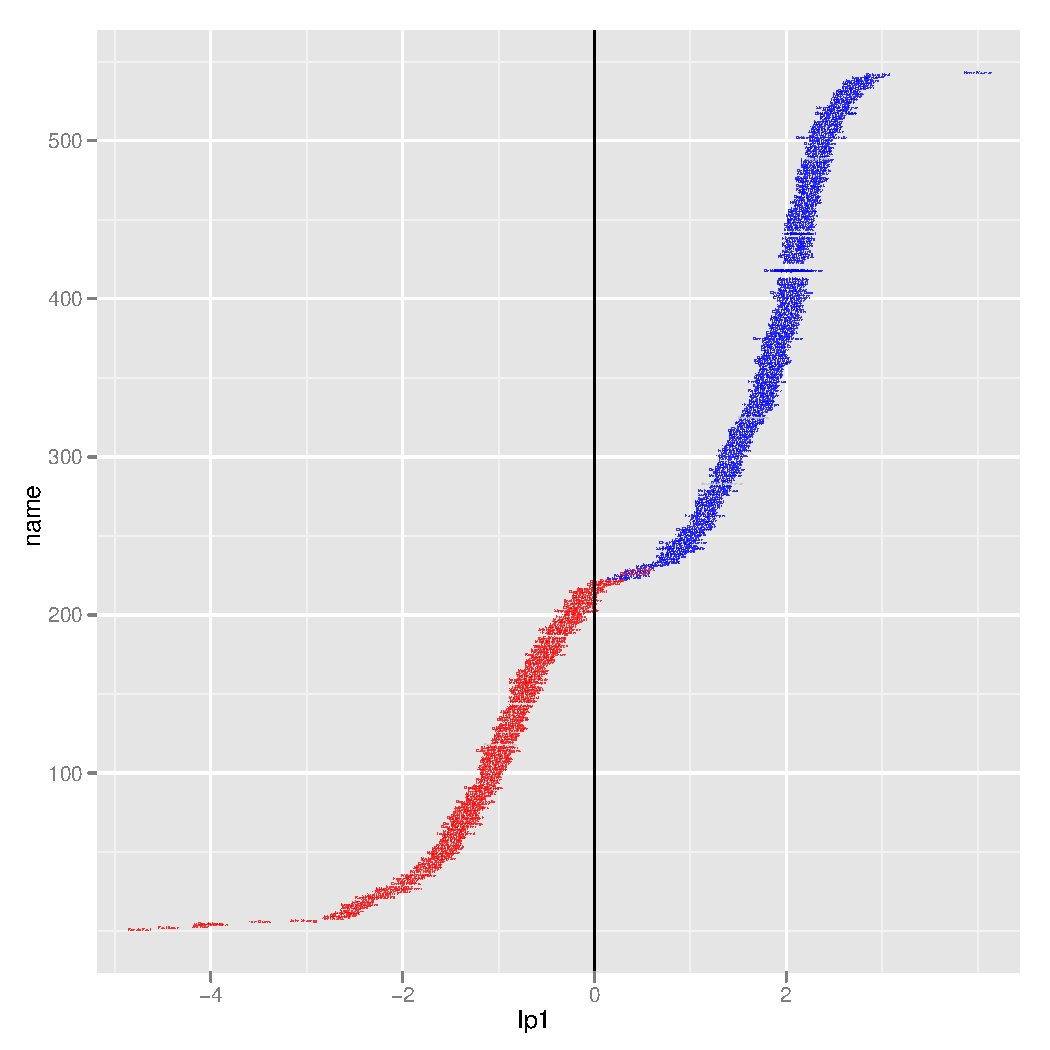
\includegraphics[width=1.\textwidth]
  {chapter_spatial_voting_with_text/figures/134_legislator_name_accuracy_by_ip.pdf}
  \caption{All legislator ideal points in the 111th Congress.  Using
    votes, ideal points can separate the U.S. political parties
    Democrats (blue) and Republicans (red).  The Y axis contains no
    information; it is used to stack names for display purposes.}
\label{fig:all_ideal_points}
\end{figure}

\begin{figure}[t]
  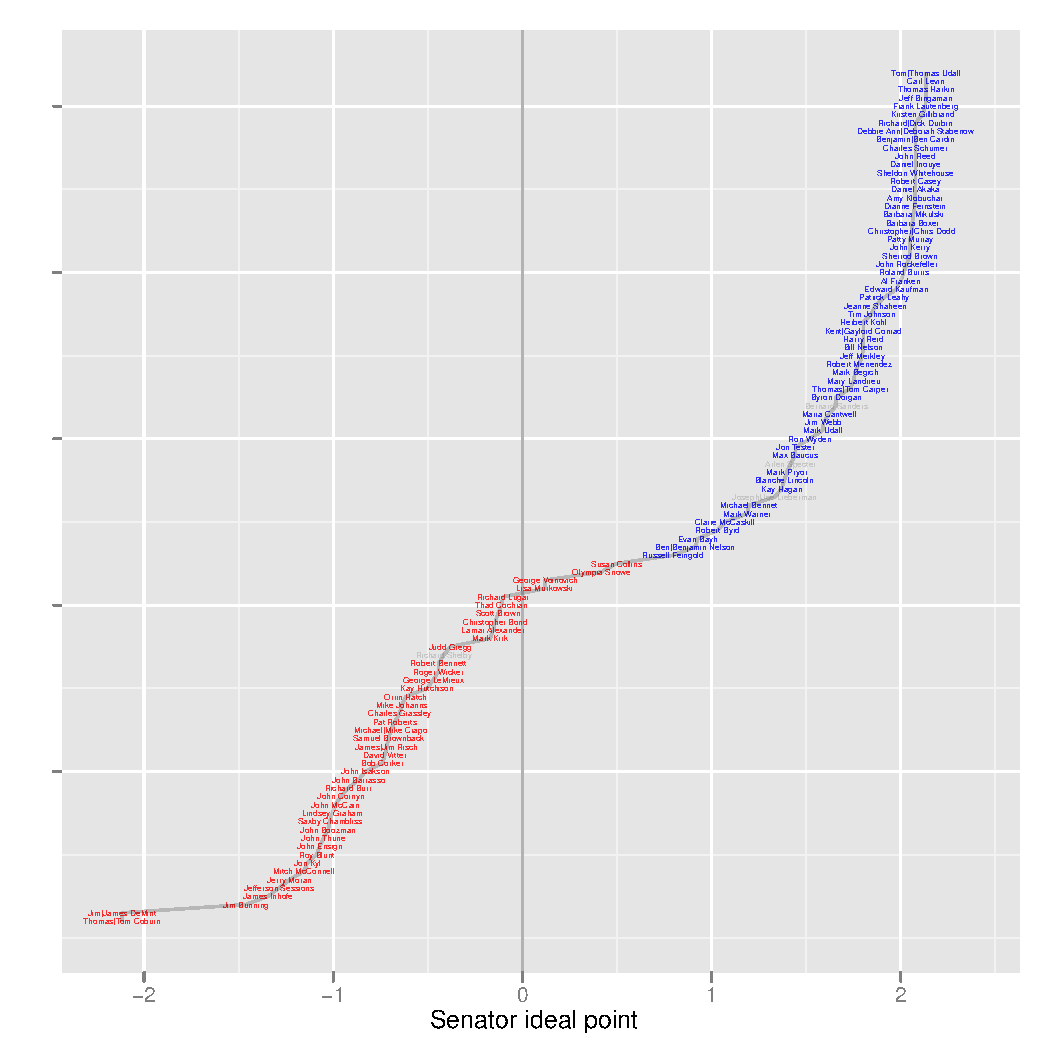
\includegraphics[width=1.\textwidth]
  {chapter_spatial_voting_with_text/figures/134_senator_name_accuracy_by_ip.pdf}
  \caption{All Senator ideal points in the 111th Congress.  Using
    votes, ideal points can separate the U.S. political parties
    Democrats (blue) and Republicans (red).}
\label{fig:senate_ideal_points}
\end{figure}


%\markright{{\bf DRAFT COPY: DO NOT CITE OR DISTRIBUTE}}
% \pagestyle{myheadings}


%% \section*{Acknowledgments}

%% \bibliographystyle{naaclhlt2010/naaclhlt2010}
%% \bibliography{../bib.bib}

%% \end{bill}


\section{Additional notes for the Issue-Adjusted Ideal Point Model}
\subsection*{Sparsity.}
Issue adjustments $\bm z_u$ ranged widely, moving some lawmakers
significantly. The variational estimates were not sparse, although a
high mass was concentrated around 0. Twenty-nine percent of issue
adjustments were within $[-0.01, 0.01]$, and eighty-seven percent of
issue adjustments were within $[-0.1, 0.1]$.

\subsection*{Hyperparameter settings}
The most obvious parameter in the issue voting model is the
regularization term $\lambda$. The Bayesian treatment described in
the Inference section of \emph{How they Vote} demonstrated considerable robustness
to overfitting at the expense of precision.  With $\lambda=0.001$,
for example, issue adjustments $z_{uk}$ remained on the order of single digits,
while the MAP estimate yielded adjustment estimates over 100.

We recommend a modest value of $1 < \theta < 10$.  At this value, the model
outperforms ideal points in validation experiments on both the House
and Senate while maintaining stability in the two-stage model.

\subsection*{Implementation.}
%% %% This was not a problem in more recent runs.
%% In rare circumstances, the variational and MAP estimates
%% resulted in degenerate solutions, in which the model performed no
%% better than assuming lawmakers vote \verb!yea!.  When we reran these
%% experiments, the solution was no longer degenerate (this did not
%% affect the reported median accuracy in
%% Table~\ref{table:median_accuracy}).

When performing the second-order updates described in
the Inference section, we skipped variable updates when the
estimated Hessian was not positive definite (this disappeared when
sample sizes grew large enough).  We also limited step sizes to 0.1
(another possible reason for smaller coefficients).

\subsection*{Issue labels}
\label{section:issue_issue_labels}

In the empirical analysis, we used issue labels obtained from the
Congressional Research Service.  There were $5,861$ labels, ranging
from \emph{World Wide Web} to \emph{Age}.  We only used issue labels
which were applied to at least twenty five bills in the 12 years under
consideration.  This filter resulted in seventy-four labels which
correspond fairly well to political issues.  These issues, and the
number of documents each label was applied to, is given in
Table~\ref{table:issues}.

\begin{table*}[htdp]
  \caption{Issue labels and the number of documents with each label
  (as assigned by the Congressional Research Service) for Congresses 106 to 111 (1999 to
  2010).}
  \small
  \begin{center}
  \begin{tabular}{cc}
    \rowcolors{1}{gray!30}{}
  \begin{tabular}{|p{5.8cm}|p{.7cm}|}
    \hline
    \textcolor{black} {} \textbf{Issue label} & \textcolor{black} {}\textbf{Bills} \\ 
    \hline
\textcolor{black} {}    Women & \textcolor{black}{}25  \\ \textcolor{black} {}
    Military history & \textcolor{black}{}25  \\ \textcolor{black} {}
    Civil rights & \textcolor{black}{}25  \\ \textcolor{black} {}
    Government buildings; facilities; and property & \textcolor{black}{}26  \\ \textcolor{black} {}
    Terrorism & \textcolor{black}{}26  \\ \textcolor{black} {}
    Energy & \textcolor{black}{}26  \\ \textcolor{black} {}
    Crime and law enforcement & \textcolor{black}{}27  \\ \textcolor{black} {}
    Congressional sessions & \textcolor{black}{}27  \\ \textcolor{black} {}
    East Asia & \textcolor{black}{}28  \\ \textcolor{black} {}
    Appropriations & \textcolor{black}{}28  \\ \textcolor{black} {}
    Business & \textcolor{black}{}29  \\ \textcolor{black} {}
    Congressional reporting requirements & \textcolor{black}{}30  \\ \textcolor{black} {}
    Congressional oversight & \textcolor{black}{}30  \\ \textcolor{black} {}
    Special weeks & \textcolor{black}{}31  \\ \textcolor{black} {}
    Social services & \textcolor{black}{}31  \\ \textcolor{black} {}
    Health & \textcolor{black}{}33  \\ \textcolor{black} {}
    Special days & \textcolor{black}{}33  \\ \textcolor{black} {}
    California & \textcolor{black}{}33  \\ \textcolor{black} {}
    Social work; volunteer service; charitable organizations & \textcolor{black}{}33  \\ \textcolor{black} {}
    State and local government & \textcolor{black}{}34  \\ \textcolor{black} {}
    Civil liberties & \textcolor{black}{}35  \\ \textcolor{black} {}
    Government information and archives & \textcolor{black}{}35  \\ \textcolor{black} {}
    Presidents & \textcolor{black}{}35  \\ \textcolor{black} {}
    Government employees & \textcolor{black}{}35  \\ \textcolor{black} {}
    Executive departments & \textcolor{black}{}35  \\ \textcolor{black} {}
    Racial and ethnic relations & \textcolor{black}{}36  \\ \textcolor{black} {}
    Sports and recreation & \textcolor{black}{}36  \\ \textcolor{black} {}
    Labor & \textcolor{black}{}36  \\ \textcolor{black} {}
    Special months & \textcolor{black}{}39  \\ \textcolor{black} {}
    Children & \textcolor{black}{}40  \\ \textcolor{black} {}
    Veterans & \textcolor{black}{}40  \\ \textcolor{black} {}
    Human rights & \textcolor{black}{}41  \\ \textcolor{black} {}
    Finance & \textcolor{black}{}41  \\ \textcolor{black} {}
    Religion & \textcolor{black}{}42  \\ \textcolor{black} {}
    Politics and government & \textcolor{black}{}43  \\ \textcolor{black} {}
    Minorities & \textcolor{black}{}44  \\ \textcolor{black} {}
    Public lands and natural resources & \textcolor{black}{}44  \\
    \hline
  \end{tabular}
   &
    \rowcolors{1}{gray!30}{}
  \begin{tabular}{|p{5.8cm}|p{.7cm}|}
    \hline
    \textcolor{black} {} \textbf{Issue label} & \textcolor{black}{}\textcolor{black} {} \textbf{Bills} \\
    \hline
    Europe & \textcolor{black}{}44  \\ \textcolor{black} {}
    Military personnel and dependents & \textcolor{black}{}44  \\ \textcolor{black} {}
    Taxation & \textcolor{black}{}47  \\ \textcolor{black} {}
    Government operations and politics & \textcolor{black}{}47  \\ \textcolor{black} {}
    Postal facilities & \textcolor{black}{}47  \\ \textcolor{black} {}
    Medicine & \textcolor{black}{}48  \\ \textcolor{black} {}
    Transportation & \textcolor{black}{}48  \\ \textcolor{black} {}
    Emergency management & \textcolor{black}{}48  \\ \textcolor{black} {}
    Sports & \textcolor{black}{}52  \\ \textcolor{black} {}
    Families & \textcolor{black}{}53  \\ \textcolor{black} {}
    Medical care & \textcolor{black}{}54  \\ \textcolor{black} {}
    Athletes & \textcolor{black}{}56  \\ \textcolor{black} {}
    Land transfers & \textcolor{black}{}56  \\ \textcolor{black} {}
    Armed forces and national security & \textcolor{black}{}56  \\ \textcolor{black} {}
    Natural resources & \textcolor{black}{}58  \\ \textcolor{black} {}
    Law & \textcolor{black}{}60  \\ \textcolor{black} {}
    History & \textcolor{black}{}61  \\ \textcolor{black} {}
    Names & \textcolor{black}{}62  \\ \textcolor{black} {}
    Criminal justice & \textcolor{black}{}62  \\ \textcolor{black} {}
    Communications & \textcolor{black}{}65  \\ \textcolor{black} {}
    Public lands & \textcolor{black}{}68  \\ \textcolor{black} {}
    Legislative rules and procedure & \textcolor{black}{}69  \\ \textcolor{black} {}
    Elementary and secondary education & \textcolor{black}{}74  \\ \textcolor{black} {}
    Anniversaries & \textcolor{black}{}82  \\ \textcolor{black} {}
    Armed forces & \textcolor{black}{}83  \\ \textcolor{black} {}
    Defense policy & \textcolor{black}{}92  \\ \textcolor{black} {}
    Higher education & \textcolor{black}{}103  \\ \textcolor{black} {}
    Foreign policy & \textcolor{black}{}104  \\ \textcolor{black} {}
    International affairs & \textcolor{black}{}105  \\ \textcolor{black} {}
    Budgets & \textcolor{black}{}112  \\ \textcolor{black} {}
    Education & \textcolor{black}{}122  \\ \textcolor{black} {}
    House of Representatives & \textcolor{black}{}142  \\ \textcolor{black} {}
    Commemorative events and holidays & \textcolor{black}{}195  \\ \textcolor{black} {}
    House rules and procedure & \textcolor{black}{}329  \\ \textcolor{black} {}
    Commemorations & \textcolor{black}{}400  \\ \textcolor{black} {}
    Congressional tributes & \textcolor{black}{}541  \\ \textcolor{black} {}
    Congress & \textcolor{black}{}693  \\
    \hline
  \end{tabular}
  \end{tabular}
  \end{center}
  \label{table:issues}
\end{table*}

\subsection*{Corpus preparation}
\label{section:issue_corpus_preparation}
In this section we provide further details of vocabulary selection.
We began by considering all phrases with one to five words.  From
these, we immediately ignored phrases which occurred in more than
$10\%$ of bills and fewer than $4$ bills, or which occurred as fewer
than $0.001\%$ of all phrases.  This resulted in a list of 40603
phrases.

We then used a set of features characterizing each word to classify
whether it was good or bad to use in the vocabulary.  Some of these
features were based on corpus statistics, such as the number of bills
in which a word appeared.  Other features used external data sources,
including whether, and how frequently, a word appeared as link text in
a Wikipedia article. For training data, we used a manually curated
list of 458 ``bad'' phrases which were semantically awkward or
meaningles (such as \emph{the follow bill}, \emph{and sec ammend},
\emph{to a study}, and \emph{pr}) as negative examples in a
$L_2$-penalized logistic regression to select a list of 5,000 ``good''
words.

\begin{table*}
  \caption{Features and coefficients used for predicting ``good''
  phrases.  Below, $\mbox{test}$ is a test statistic which measures
  deviation from a model assuming that words appear independently;
  large values indicate that they occur more often than expected by
  chance.  We define it as $\mbox{test}=\frac{\mbox{Observed count} -
  \mbox{Expected count}}{\sqrt{\mbox{Expected count under a language
  model assuming independence}}}$.} \rowcolors{1}{gray!30}{}
\begin{center}
  \begin{tabular}{|p{6.0cm}|p{6.7cm}|p{1.0cm}|}
      \hline
  \textcolor{black} {} 
      \textbf{Coefficient} &   \textcolor{black} {} \textbf{Summary} &   \textcolor{black} {} \textbf{Weight} \\
      \hline
      \textcolor{black} {}
      log(count + 1) & \textcolor{black}{}Frequency of phrase in corpus & \textcolor{black}{}-0.018 \\ \textcolor{black} {}
      log(number.docs + 1) & \textcolor{black}{}Number of bills containing phrase & \textcolor{black}{}0.793 \\ \textcolor{black} {}
      anchortext.presentTRUE & \textcolor{black}{}Occurs as anchortext in Wikipedia & \textcolor{black}{}1.730 \\ \textcolor{black} {}
      anchortext & \textcolor{black}{}Frequency of appearing as anchortext in Wikipedia & \textcolor{black}{}1.752 \\ \textcolor{black} {}
      frequency.sum.div.number.docs & \textcolor{black}{}Frequency divided by number of bills & \textcolor{black}{}-0.007 \\ \textcolor{black} {}
      doc.sq & \textcolor{black}{}Number of bills containing phrase, squared & \textcolor{black}{}-0.294 \\ \textcolor{black} {}
      has.secTRUE & \textcolor{black}{}Contains the phrase \emph{sec} & \textcolor{black}{}-0.469 \\ \textcolor{black} {}
      has.parTRUE & \textcolor{black}{}Contains the phrase \emph{paragra} & \textcolor{black}{}-0.375 \\ \textcolor{black} {}
      has.strikTRUE & \textcolor{black}{}Contains the phrase \emph{strik} & \textcolor{black}{}-0.937 \\ \textcolor{black} {}
      has.amendTRUE & \textcolor{black}{}Contains the phrase \emph{amend} & \textcolor{black}{}-0.484 \\ \textcolor{black} {}
      has.insTRUE & \textcolor{black}{}Contains the phrase \emph{insert} & \textcolor{black}{}-0.727 \\ \textcolor{black} {}
      has.clauseTRUE & \textcolor{black}{}Contains the phrase \emph{clause} & \textcolor{black}{}-0.268 \\ \textcolor{black} {}
      has.provisionTRUE & \textcolor{black}{}Contains the phrase \emph{provision} & \textcolor{black}{}-0.432 \\ \textcolor{black} {}
      has.titleTRUE & \textcolor{black}{}Contains the phrase \emph{title} & \textcolor{black}{}-0.841 \\ \textcolor{black} {}
      test.pos & \textcolor{black}{}$\ln(max(-\mbox{test}, 0) + 1)$ & \textcolor{black}{}0.091 \\ \textcolor{black} {}
      test.zeroTRUE & \textcolor{black}{}$1$ if $\mbox{test} = 0$ & \textcolor{black}{}-1.623 \\ \textcolor{black} {}
      test.neg & \textcolor{black}{}$\ln(max(\mbox{test}, 0) + 1)$ & \textcolor{black}{}0.060 \\ \textcolor{black} {}
      number.terms1 & \textcolor{black}{}Number of terms in phrase is 1 & \textcolor{black}{}-1.623 \\ \textcolor{black} {}
      number.terms2 & \textcolor{black}{}Number of terms in phrase is 2 & \textcolor{black}{}2.241 \\ \textcolor{black} {}
      number.terms3 & \textcolor{black}{}Number of terms in phrase is 3 & \textcolor{black}{}0.315 \\ \textcolor{black} {}
      number.terms4 & \textcolor{black}{}Number of terms in phrase is 4 & \textcolor{black}{}-0.478 \\ \textcolor{black} {}
      number.terms5 & \textcolor{black}{}Number of terms in phrase is 5 & \textcolor{black}{}-0.454 \\ \textcolor{black} {}
      log(number.docs + 1) * anchortext & \textcolor{black}{}$\ln(\mbox{Number of bills containing phrase})$
      $\times 1_{\{ \mbox{Appears in Wikipedia anchortext} \}}$ & \textcolor{black}{}-0.118 \\ \textcolor{black} {}
      log(count + 1) * log(number.docs + 1) & \textcolor{black}{}$\ln(\mbox{Number of bills containing phrase} + 1)$
      $\times \ln(\mbox{Frequency of phrase in corpus} + 1)$ & \textcolor{black}{} 0.246 \\
      \hline
    \end{tabular}
    \end{center}
\end{table*}


\section{Improving convergence of stochastic optimization}

\subsection{Round-robin updates}

\subsection{Bounded step size}

\chapter{Notes on the analysis of text data}
\label{chapter:notes_text}
\section{Processing text data}

\subsection{Stemming and parsing}

\subsection{Current libraries and software}

\section{Model estimation basics}

\subsection{Multimodal distributions and identification}

\subsection{Setup of a typical program}

\subsection{The role of traditional dimensionality reduction in evaluating underconstrained distributions}
